%\documentclass[10pt,twocolumn,letterpaper,draft]{article}
\documentclass[10pt,letterpaper]{ctexart}

\usepackage{cvpr}
\usepackage{graphicx}
\usepackage{wrapfig}
\usepackage{amsmath}
\newtheorem{myDef}{Definition}
\newtheorem{myTheo}{Theorem}

\usepackage{amssymb}
\usepackage{booktabs}
\usepackage{subfigure}
\usepackage{algorithm}
\usepackage{algorithmicx}
\usepackage{algpseudocode}
\usepackage{pythonhighlight}
\usepackage{xcolor}
\usepackage{listings}

\lstset{language=C++,
    basicstyle=\ttfamily,
    frame=single,
    keywordstyle=\color{blue}\ttfamily,
    stringstyle=\color{magenta}\ttfamily,
    commentstyle=\color{green}\ttfamily,
    morecomment=[l][\color{magenta}]{\#},
    morekeywords={*,uint_fast64_t}
}

\renewcommand{\labelenumi}{\alph{enumi}.} % Make numbering in the enumerate environment by letter rather than number (e.g. section 6)
\floatname{algorithm}{算法}
\renewcommand{\algorithmicrequire}{\textbf{输入:}}
\renewcommand{\algorithmicensure}{\textbf{输出:}}
\renewcommand{\lstlistingname}{代码清单}

\usepackage{enumitem}
\setenumerate[1]{itemsep=0pt,partopsep=0pt,parsep=\parskip,topsep=5pt}
\setitemize[1]{itemsep=0pt,partopsep=0pt,parsep=\parskip,topsep=5pt}
\setdescription{itemsep=0pt,partopsep=0pt,parsep=\parskip,topsep=5pt}

% Include other packages here, before hyperref.

% If you comment hyperref and then uncomment it, you should delete
% egpaper.aux before re-running latex.  (Or just hit 'q' on the first latex
% run, let it finish, and you should be clear).
\usepackage[pagebackref=true,breaklinks=true,letterpaper=true,colorlinks,bookmarks=false]{hyperref}


\cvprfinalcopy % *** Uncomment this line for the final submission

\def\cvprPaperID{159} % *** Enter the CVPR Paper ID here
\def\httilde{\mbox{\tt\raisebox{-.5ex}{\symbol{126}}}}

\newcommand{\mypara}[1]{\paragraph{#1.}}

\graphicspath{{figures/}}

% Pages are numbered in submission mode, and unnumbered in camera-ready
%\ifcvprfinal\pagestyle{empty}\fi
\setcounter{page}{1}


%\begin{CJK*}{GBK}{song}

\newcommand{\figref}[1]{图\ref{#1}}
\newcommand{\tabref}[1]{表\ref{#1}}
\newcommand{\equref}[1]{式\ref{#1}}
\newcommand{\secref}[1]{第\ref{#1}节}

\ctexset{
  section={
          name={,、},
          number={\chinese{section}},
          format={\heiti},
          beforeskip={0.1ex},
          afterskip={0.1ex},
          aftername={\nobreak},
          indent={\parindent},
          },
}
\usepackage{zhnumber}

\newcommand\zhsubsec[1]{{% 中文小节
\bfseries{
\stepcounter{subsection}(\zhnum{subsection}){#1}}
\vspace{0.1pt}%
}}

%%%%%%%%% TITLE

\begin{document}
\pagestyle{plain}
\title{
    \begin{center}
        \phantom{Start!}
    	  \vspace{2cm}
        \center{\zihao{1} 中山大学数据科学与计算机学院}
        \center{\zihao{2} 程序设计与数据结构综合实践II}
        \center{\zihao{2} TSP问题实验报告}
        \center{(2018-2019学年秋季学期)}
    \end{center}
}
\maketitle

\begin{center}
    \setlength{\baselineskip}{40pt}
    \vspace{1cm}
    \zihao{-2}
    \center{
        \begin{tabular}{cc}
      	学\qquad 号:& \underline{~~~~~~16337113~~~~~~}  \\
      	姓\qquad 名:& \underline{~~~~~~~劳马东~~~~~~~}  \\
      	专\qquad 业:& \underline{~~~~~~~~~超算~~~~~~~~}  \\
      	\end{tabular}
    }
\end{center}
\pagebreak

%%%%%%%%% BODY TEXT %%%%%%%%%%%%%%%%%%%%%%%%%%%%%%%%%%%%%%%%
\section{实验题目}
完成下列三项任务:
\begin{itemize}[itemindent=2em]
  \item 实现一个高效的无向简单图的TSP算法,在小规模内有精确最优解,对较大的规模能有近似解;
  \item 生成求解输入,不仅可以用于测试自己的程序,也能给其他组的同学出题,比较求解速度和结果精确度;
  \item 检验输出是否合法,是否能在图中完成TSP任务,并且路程计算无误。
\end{itemize}
\par 输入:第一行为n,接下来是n乘n的矩阵,表示两点之间的距离,示例如下:
\begin{table}[!htbp]
  \centering
  \begin{tabular}{cccc}
    4&&&\\
    0 &1& 2& 3\\
    1 &0 &4 &5\\
    2 &4 &0 &6\\
    3 &5 &6 &0\\
  \end{tabular}
\end{table}

输出:第一行为解的总路程,第二行为路径过程。
如上图可给出的解为:
\begin{table}[!htbp]
  \centering
  \begin{tabular}{ccccc}
    14&&&&\\
    0 &1& 2& 3&0\\
  \end{tabular}
\end{table}
\par 表示总路程为14(1+4+6+3),路径为0->1->2->3->0。
\section{实验内容}
  \zhsubsec {分支定界算法求解TSP精确解}
  \par 分支定界算法(branch and bound)是一种有信息搜索算法。每个节点
  的估计值由两部分组成:节点的实际代价和启发值,即:
  \begin{equation}
    f(x) = g(x) + h(x)
  \end{equation}
  其中$g(x)$是节点的当前实际路径消耗,$h(x)$是节点$x$到终点的启发值。
  \par 假设邻接矩阵的权值如下:
  \begin{equation}
    C(i, j) = 
    \begin{cases}
      W(i, j)& \text{i != j}\\
      INFINITY& \text{i == j}
    \end{cases}
  \end{equation}
  例如\figref{fig:M}的邻接矩阵$M$。
  \begin{figure}[H]
    \centering
    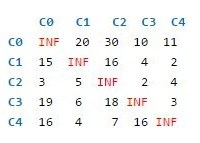
\includegraphics{M.jpg}
    \caption{CSP完全图示例}
    \label{fig:M}
  \end{figure}
  \par 有信息搜索算法(如A*和IDA*)的细节不再细写,在《人工智能》课程
  上已经有了很好的理解。下面主要讲算法的启发函数,如何计算一个节点的估计代价呢?
  使用下面的方法:对于邻接矩阵的每一行、每一列,找到对应行、列的最小值,
  节点的启发函数值就是这些最小值的和,即:
  \begin{equation}
    g(x) = \sum_{i=1}^N(min(row_i) + min(column_i)) 
  \end{equation}。
  \par 从父节点到子节点的行动如何表示呢?例如,要从城市$i$移动到城市$j$,邻接矩阵如何改变?
  首先,我们把城市$i$的所有出边置为INFINITY,把城市$j$的所有入边置为INFINITY,把城市$j$到城市0
  的边置为INFINITY。然后,对矩阵的每一行、每一列,执行一个松弛操作:减去对应的最小值,最终使每一行、
  每一列有至少一个值为0。例如,从城市0移动到城市1,\figref{fig:move_c}中红色标注的元素被置为INFINITY,
  变成\figref{fig:move_c}。除此之外,行动会导致邻接矩阵被松弛:每一行、每一列减去对应的最小值,
  最终导致每一行、列至少有一个权值为0。
  \begin{figure}[H]
    \centering
    \subfigure[父节点M]{
      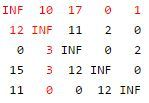
\includegraphics[width=0.3\textwidth]{M_p.jpg}
      \label{fig:move_p}
    }
    \subfigure[子节点M]{
      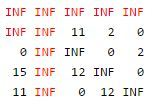
\includegraphics[width=0.3\textwidth]{M_c.jpg}
      \label{fig:move_c}
    }
    \caption{置INFINITY示例}
  \end{figure}
  \begin{algorithm}
      \caption{节点间的行动}
      \begin{algorithmic}[1] %每行显示行号
        \Require $from, to$:城市编号,$M$:城市$from$的$n \times n$邻接矩阵
          \Function {move}{$from, to, M$}
            \State $n \gets$ M.size()
            \For{$i \in [0, n)$}
              \State $M[from][i] \gets M[i][to] \gets INFINITY$
            \EndFor
            \State $M[to][0] \gets INFINITY$
            \State reduceRow($M, n$)
            \State reduceCol($M, n$)
          \EndFunction
      \end{algorithmic}
  \end{algorithm}

  \begin{algorithm}
    \caption{A*算法}
    \begin{algorithmic}[1] %每行显示行号
        \Function {move}{$M$}
          \State $heap$:以节点估计值存储的最小堆
          \State $root \gets$ Node($0$)
          \State $root.cost \gets$ heuristic($M$)
          \State move($-1, 0, M$)
          \State $root.matrix \gets M$
          \State $heap$.push($root$)
          \While{$heap$ is not empty}
            \State $best \gets heap.$pop()
            \For {\textbf{each} neighbor $v$ of $best$}
              \State $new\_node \gets$ Node($v$)
              \State $M\_tmp \gets$ copy($best.matrix$)
              \State $new\_node.cost \gets best.cost + M\_tmp[best.num][v] +$ heuristic($M\_tmp$)
              \State move($best.num, v, M\_tmp$)
              \State $new\_node.matrix \gets M\_tmp$
              \State $heap$.push($new\_node$)
            \EndFor
          \EndWhile
        \EndFunction
    \end{algorithmic}
\end{algorithm}

  \zhsubsec {生成输入}
  \par 城市与城市之间的权值随机确定,由于城市到自己没有路径,而且问题是针对无向图的,因此需要使用一个
  二维矩阵来存储随机结果,以保证$M[i][j]==M[j][i]$。

  \newpage
  \zhsubsec {输出检验}
  \par 检验包括四个方面:输出结果是否涵盖所有城市?是不是每个城市只经过1次?顺着输出结果能不能走
  到起点?路径代价的精确度如何?
  \par 对于第一个问题,使用一个全集,每经过一个城市就从集合中删除一个城市,最终集合为空时假设成立。
  \par 对于第二个问题,使用一个统计数组,如果发现某个元素不等于1,假设不成立。
  \par 对于第三个问题,顺着输出结果在图上走,如果发现边不合法,输出错误;结果的最后一个值必须与第一个值相同。
  \par 上一步可以统计路径的权值,将其和暴力搜索的结果相比,判断是否相等(需要精确解时)或计算精度(需要近似解时)。

\newpage
\section{关键代码}
\begin{enumerate}[itemindent=2em,label=\arabic*、]
  \item 分支定界算法A*部分
  \begin{lstlisting}[caption=A*,label={code:read},captionpos=b]
pair<int, vector<int>> solve(vector<vector<int>>& cost_matrix) {
    ...
    Node *root = new Node(cost_matrix, path, 0, -1, 0);
    pq.push(root);    // pq是以节点的lower_bound值排序的最小堆
    while (!pq.empty()) {
        Node *best = pq.top();    // 取当前f(x)最小的一个
        pq.pop();
        if (best->level == n - 1) // 找到解
        else {
            for (int j = 0; j < n; ++j) {
                int w = best->reduced_matrix[best->vertex][j];
                if (w != INF) {
                    // 扩展节点,由于做了松弛,总的估计值还需加上父节点启发值
                    Node *child = new Node(best->reduced_matrix, best->path,
                            best->vertex, j, best->lower_bound + w);
                    pq.push(child);
                }
            }
        }
    }
    ...
}
  \end{lstlisting}

  \item 分支定界算法计算启发值与松弛
  \begin{lstlisting}[caption=创建节点,label={code:read},captionpos=b]
Node(vector<vector<int>> m, vector<pair<int, int>> p,
     int from, int to, int g=0): path(p), reduced_matrix(m), vertex(j) {
    ...
    if (from > -1) {      // 第from行、to列置为INF
        for (int k = 0; k < n; ++k) {
            reduced_matrix[from][k] = reduced_matrix[k][to] = INF;
        }
    }
    reduced_matrix[to][0] = INF;    // 节点到起点的边置为INF
    // heuristic计算启发值,然后对行和列执行reduce操作
    lower_bound = g + heuristic(reduced_matrix);
}
  \end{lstlisting}
\end{enumerate}

\section{实验结果}
\begin{figure}[H]
  \centering
  \subfigure[输入1]{
    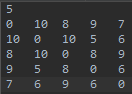
\includegraphics[width=0.3\textwidth]{input.png}
  }
  \subfigure[输入2]{
    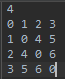
\includegraphics[width=0.175\textwidth]{input2.png}
  }
  \\
  \subfigure[输出1]{
    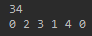
\includegraphics[width=0.2\textwidth]{output.png}
  }
  \subfigure[输出2]{
    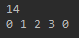
\includegraphics[width=0.17\textwidth]{output2.png}
  }
\end{figure}

\begin{table}[!htbp]
  \centering
  \begin{tabular}{cc}
    \toprule
    n & 时间/s\\
    \midrule
    5 & 0\\
    10 & 0.013\\
    15 & 0.736\\
    20 & 21.836\\
    \bottomrule
  \end{tabular}
  \caption{运行时间}
\end{table}
\end{document}
